\section{Méthodes de Détection des Valeurs Aberrantes}\label{Section:2}
% par Richard Millson
\subsection{Méthodes basées sur la distance}

Pour déterminer si un point est anormal, il doit être comparé à un ensemble d'autres points. 
Une comparaison naturelle serait de considérer sa distance par rapport aux autres,
avec la distance croissante des autres étant de plus en plus suggestive, c'est une anomalie.
Cette approche fonctionne à la fois dans les cas continus et discrets chaque fois qu'on nous donne soit une fonction de distance, soit un tableau pré-calculé de distances par paires.
Le choix des ensembles de points à utiliser dans cette comparaison distingue les différents algorithmes basés sur la distance.

Cette discussion commence par l'introduction d'une notation.
Soit $D \subset \mathbb{R}^n$ un ensemble de données à dimension $n$, 
$p$ et $q$ sont des points de données à partir de $D$, 
$P \subset D$ être un sous-ensemble de $D$, 
et $d : D \times D \to \mathbb{R}$ est la distance entre $p$ et $q$ écrit $d(p,q)$.
Un algorithme de détection d'anomalie doit nous donner une fonction $a : D \to \mathbb{R}$ qui décrit l'anomalie d'un point donné.
Cela induit un ordonnancement sur les points de $D$ ;
si $a(p) < a(q)$ pour $p,q \in D$, alors $p$ est moins anormal que $q$.
Il est alors nécessaire de définir un seuil au-delà duquel un point est considéré comme anormal.
Si $\alpha \in \mathbb{R}$ est un tel seuil, alors tout $p \in D$ où $a(p) > \alpha$ est considéré comme une anomalie.
De tels $p$ sont appelés \textbf{absolument anormaux}.

\subsubsection*{Mesures de similarité}

Une \textbf{mesure de similarité} est une fonction à valeur réelle qui décrit la similarité entre deux objets.
Une construction courante consiste à définir la similarité entre deux points comme $\frac{1}{d(p,q)}$ pour une fonction de distance $d$.

Une mesure de similarité peut également être construite entre des distributions de probabilités.
Soit $X$ et $Y$ deux vecteurs aléatoires de dimension $n$ de distribution (éventuellement) différente avec pmfs $f_X$ et $f_Y$ respectivement.
Soit $\Omega$ leur domaine partagé.
La \textbf{distance de Bhattacharyya } est définie comme étant 
\[
-\ln\left( \sum_{z \in \Omega} \sqrt{f_X(z) f_Y(z)} \right)
\]
Il peut être étendu pour le cas où $X$ et $Y$ sont continus. On peut aussi considérer la distance de Bhattacharyya entre la distribution du point et une autre distribution.
Ce cas particulier est appelé la \textbf{Distance de Mahalanobis}.

\[
\sqrt{(p - q)^T \Sigma^{-1} (p - q)}
\]
ou $\Sigma$ matrice de covariance.

Si $\Sigma$ est diagonale, alors  
la distance de Mahalanobis. devient

\[
\sqrt{\sum_{i=1}^n \frac{(p_i - q_i)^2}{\sigma_i^2}}
\]
où $\sigma_i^2$ est la $i$ ième écart-type.
Si $\Sigma$ est la matrice d'identité, alors on récupère la \textbf{Distance euclidienne}

\[
\sqrt{\sum_{i=1}^n (p_i - q_i)^2}
\]

En prenant la distance euclidienne, une normalisation linéaire peut d'abord être appliquée à chaque dimension de sorte que chaque entrée se situe entre $[-1,1]^n$.

La \textbf{Distance de Minkowski} d'ordre $p$ est définie comme

\[
\left( \sum_{i=1}^d |p_i - q_i|^p \right)^{1/p}
\]

Pour $p=2$ on récupère le \textbf{distance euclidienne},
et pour $p=1$ on récupère le \textbf{la distance de Manhattan}.
Cette distance est une métrique pour $p \geq 1$ 
(et peut en fait être définie en fonction de la norme $p$ d'un espace $L^p$).
Considérer la limite comme $p$ va à l'infini donne la distance \textbf{Chebyshev} (aussi appelée la métrique $L^\infty$) définie par
\[
\max_{i=1}^d |p_i - q_i|
\]
et en considérant la limite comme $p$ va à l'infini négatif donne
\[
\min_{i=1}^d |p_i - q_i|
\]
Pour deux ensembles de données $P$ et $Q$, leur \textbf{similarité de Jaccard} est définie comme la taille de leur intersection divisée par la taille de leur union
\[
J(P, Q)
= \frac{|P \cap Q|}{|P \cup Q|}
= \frac{|P \cap Q|}{|P| + |Q| - |P \cap Q|}
\]
Leur \textbf{distance de Jaccard} est alors considéré comme $1 - J(P, Q)$.

Cette définition peut être étendue pour comparer des vecteurs binaires (c'est-à-dire des vecteurs avec des entrées de seulement des uns et des zéros) de même longueur.
Étant donné deux vecteurs binaires $p$ et $q$ de longueur $d$, considérons un ensemble arbitraire d'éléments $d$ $D$.
Alors $p$ et $q$ peuvent être considérés comme des sous-ensembles de $D$ ; si $p_i=1$ alors on peut dire que $p$ contient le $i$-ième élément de $D$, et si $p_i=0$ alors il n'inclut pas ce $i$-ième élément.
En regardant $p$ et $q$ de cette façon, leur similarité de Jaccard peut être calculée comme ci-dessus.

Que $p$ et $q$ soient deux vecteurs non nuls.
Rappelez-vous que 
$p \cdot q 
= \lVert p \rVert \lVert q \rVert \cos\theta$
où $\theta$ est l'angle entre $p$ et $q$.
Ensuite, le \textbf{Similitude du cosinus} est considéré comme le cosinus de cet angle, qui peut être calculé comme
\[
\cos\theta
= \frac{p \cdot q}{\lVert p \rVert \lVert q \rVert}
= \frac{\sum_{i=1}^d p_i q_i}{\sqrt{\sum_{i=1}^d p_i^2} \sqrt{\sum_{i=1}^d q_i^2}}
\]
Cette valeur varie entre 1 et -1, 1 étant atteint lorsque $p=q$, -1 lorsque $p=-q$, et 0 lorsque $p$ et $q$ sont perpendiculaires.

\subsubsection*{Approches fondées sur la distance}

Ces fonctions de distance peuvent être appliquées pour créer quelques algorithmes de base de détection d'anomalies.
Ces idées seront ensuite étendues à des algorithmes plus complexes.

Étant donné une fonction de distance $d$ et un jeu de données $D$, 
l'algorithme de détection d'anomalie \textbf{distance à tous les points} considère chaque point $p$ en $D$ et additionne la distance de $p$ à chaque autre point en $D$, c'est-à-dire
\[
a(p) 
= \sum_{q \in D, q \not= p} d(q, p)
\]
Le point qui maximise $a$ est alors dit anormal.
Notez que la valeur la plus extrême sera souvent considérée comme anormale, ce qui n'est pas forcément très révélateur.

L'algorithme \textbf{distance au plus proche voisin} est défini intuitivement
\[
a(p) 
= \min_{q \in D, q \not= p} d(q, p)
\]
Les paramètres \textbf{distance moyenne aux $k$ voisins les plus proches} et \textbf{distance médiane aux $k$ voisins les plus proches} sont également simples à définir.

\subsection{Méthodes basées sur la densité} % p97

Les approches fondées sur la densité considèrent les points comme anormaux s'ils se trouvent dans une région à faible densité.
% Three density-based methods are presented in this section, however there are many 

\subsubsection*{Local Outlier Factor (LOF)} % p110

\begin{algorithm}[ht]
\SetAlgoLined
\textbf{Entrée:} jeu de données $D$, point $p \in D$, entier $k$ pour le nombre de voisins les plus proches à considérer, fonction de distance $d$
\\ Calculer la distance mutuelle entre tous les points en $D$
\\\For{$p \in D$}{
\For{$q \in D \setminus \{p\}$}{
Calculer $d(p, q)$
}
Ordonner $D$ en augmentant la distance à partir de $p$
\\Poser $d_k(p) = d(p, q_k)$
}
Trouvez les $k$ les plus proches voisins de $p$ 
\\(acceptant plus de $k$ s'il y a égalité)
\\ Poser $N_k(p) = \{ q \in D \setminus \{p\} : d(p, q) \leq d_k(p) \}$
\\ Définir la distance d'accessibilité
$d_{reach}(p,q) = \max\{d_k(q), d(p,q)\}$
\\ Définir la distance moyenne d'accessibilité $\overline{d_{reach}}(p) 
= \frac{\sum_{q \in N_k(p)} d_{reach}(p,q)}{\lvert N_k(p) \rvert}$
\\Définir la densité d'accessibilité locale
$\ell_k(p) = \left( \overline{d_{reach}}(p) \right)^{-1}$
\\Calculer le local outlier factor
$a_k(p)
= \frac{\sum_{q \in N_k(p)} \frac{\ell_k(q)}{\ell_k(p)}}{\lvert N_k(p) \rvert}$
\\ \textbf{Sortie:} LOF $a_k(p)$
% \KwResult{Result}
\caption{Local Outlier Factor (LOF)}
\end{algorithm}

Le Local Outlier Factor (LOF) a été proposé en 2000 par la \cite{LOF} et a été résumé à la section 6.4.2 de la \cite{A10}.
Le LOF fonctionne en mesurant l'écart local de chaque point d'un ensemble de données par rapport à ses voisins les plus proches en $k$,
avec un point dit anormal si cette déviation est importante.
Une région locale autour d'un point $p$ est donnée en considérant les $k$ voisins les plus proches de $p$.
La densité des points dans chacun de leurs quartiers respectifs est alors estimée.
Enfin, la densité du quartier de $p$ est comparée aux densités des quartiers de chaque point dans son quartier.
On peut ensuite utiliser cette comparaison pour identifier les valeurs aberrantes qui habitent des régions de plus faible densité que leurs voisins,
par exemple $p$ dans la figure \ref{lofoutlier}.

\begin{figure}[H]
\centering
\begin{tikzpicture}
\filldraw[black] (0,0) circle (2pt) node[anchor=west] {$p$};
\draw[dashed] (0,0) circle (2);
\filldraw[black] (1.6,0.2) circle (2pt);
\filldraw[black] (2,0.834429) circle (2pt);
\draw[dashed] (1.6,0.2) circle (0.75);
\filldraw[black] (2,0) circle (2pt);
\filldraw[black] (2.5,0) circle (2pt);
\draw[dashed] (2,0) circle (0.5);
\end{tikzpicture}
\caption{Pour $k=2$, $p$ est une valeur aberrante car sa densité est plus faible que celle de ses voisins}
\label{lofoutlier}
\end{figure}

LOF introduit l'idée d'une distance d'accessibilité pour améliorer la stabilité des résultats au sein des groupes. 
Dans la figure \ref{reachability} avec $k=3$ les points $q_1, q_2, q_3$ ont tous la même distance d'accessibilité de $p$ car ils sont tous voisins de $k$.
C'est-à-dire, 
$
d_{reach}(p, q_1) 
= d_{reach}(p, q_2)
= d_{reach}(p, q_3)
= d(p, q_3)
$.
Le point  $q_4$ a 
$d_{reach}(p, q_4)
= d(p, q_4)
$
car ce n'est pas un voisin de $k$ de $p$.

\begin{figure}[H]
\centering
\begin{tikzpicture}
\filldraw[black] (0,0) circle (2pt) node[anchor=west] {$p$};
\filldraw[black] (1,0) circle (2pt) node[anchor=west] {$q_1$};
\filldraw[black] (1,-1) circle (2pt) node[anchor=west] {$q_2$};
\filldraw[black] (0,2) circle (2pt) node[anchor=north] {$q_3$};
\filldraw[black] (2,2) circle (2pt) node[anchor=west] {$q_4$};
\draw[dashed] (0,0) circle (2);
\end{tikzpicture}
\caption{La région de la distance d'accessibilité uniforme autour de $p$ pour $k=3$}
\label{reachability}
\end{figure}

LOF possède les avantages suivants:
\begin{enumerate}
\item En considérant les densités locales, il est possible d'identifier les valeurs aberrantes locales.
\end{enumerate}

LOF a les inconvénients suivants:
\begin{enumerate}
\item Il peut être difficile de sélectionner un seuil au-delà duquel un point est considéré comme une valeur aberrante.
\end{enumerate}

\subsubsection*{DBSCAN}

\begin{algorithm}[h]
\SetAlgoLined
\textbf{Entrée:} jeu de données $D$,
fonction de distance $d$,
rayon du voisinage $r>0$,
nombre minimum de points pour être considéré comme un groupe $m\in\mathbb{N}$
\\$Clusters = \{\}$
\\$Outliers = \{\}$
\\\For{$p \in D$}{
\If{$p \in Outliers \cup \left( \cup_{C \in Clusters} C \right)$}{
\textbf{continue}
}
Poser $N(p) = \{ q \in D : d(p,q) \leq r \}$
\\\If{$|N(p)| < m$}{
Ajouter $p$ à $Outliers$
\\\textbf{continue}
}
\Else{
$Cluster = N(p)$
\\\For{$q \in Cluster \setminus \{p\}$}{
\If{$q \in Outliers$}{
Enlever $q$ de $Outliers$
}
\ElseIf{$q \in \cup_{C \in Clusters} C$}{
\textbf{continue}
}
Poser $N(q) = \{ q' \in D : d(q,q') \leq r \}$
\\\If{$|N(q)| \geq m$}{
$Cluster = Cluster \cup N(q)$
}
}
}
Ajouter $Cluster$ à $Clusters$
}
retourner $Outliers$
\\\textbf{Sortie: une liste de valeurs aberrantes qui n'appartiennent à aucun groupe}
\caption{DBSCAN}
\end{algorithm}

Le regroupement spatial basé sur la densité des applications avec bruit (DBSCAN) a été proposé en 1996 par \cite{DBSCAN} et a été résumé dans la section 4.1.5 de \cite{A10}.
Comme son nom l'indique, il s'agit d'un algorithme de regroupement basé sur la densité qui regroupe les points proches et étiquette les points éloignés des autres comme des anomalies.
Le DBSCAN hiérarchique (HDBSCAN) \cite{HDBSCAN} a été introduit en 2013 et supprime le problème du choix du paramètre pour le rayon d'un voisinage en considérant tous les rayons possibles.
Une documentation supplémentaire est disponible à \cite{HDBSCAN_code}.

\begin{figure}[H]
\centering
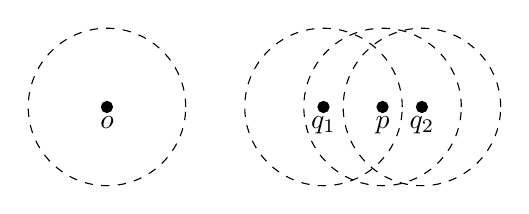
\begin{tikzpicture}
\filldraw[black] (-3.5,0) circle (2pt) node[anchor=north] {$o$};
\draw[dashed] (-3.5,0) circle (1);
\filldraw[black] (0,0) circle (2pt) node[anchor=north] {$p$};
\draw[dashed] (0,0) circle (1);
\filldraw[black] (-0.75,0) circle (2pt) node[anchor=north] {$q_1$};
\draw[dashed] (-0.75,0) circle (1);
\filldraw[black] (0.5,0) circle (2pt) node[anchor=north] {$q_2$};
\draw[dashed] (0.5,0) circle (1);
\end{tikzpicture}
\caption{Pour la taille minimale de voisinage $m=2$ et de rayon fixe $r$, $o$ est une valeur aberrante, $p$ un point central, et $q_1$ et $q_2$ des points de frontière}
\label{DBSCANlabels}
\end{figure}

Un point $p$ est un \textbf{point central} s'il y a un nombre minimum $m$ de points à l'intérieur d'une distance $r$ de $p$.
Un point $q$ est un \textbf{point frontière} s'il n'est pas lui-même un point central mais est à une distance $r$ de l'un d'eux.
Un point $o$ est une valeur aberrante s'il n'est \textbf{ni un point central ni un point frontière.}

DBSCAN considère chaque point de l'ensemble de données individuellement.
Si ce point est une valeur aberrante, il est alors ajouté à une liste de valeurs aberrantes.
Sinon, si c'est un point central, alors son voisinage $r$ forme le début d'un nouveau cluster.
Chaque point du voisinage de $r$ est alors considéré à son tour, les  voisinages  des autres points centraux contenus dans le quartier étant ajoutés à la grappe.
Cette expansion se répète jusqu'à ce que tous les points aient été examinés.
Au cours de cette étape, les points qui étaient auparavant étiquetés comme des valeurs aberrantes peuvent être mis à jour à mesure qu'ils deviennent des points frontières dans ce nouveau groupe.
Ce processus se poursuit jusqu'à ce que chaque point ait été soit attribué à un groupe, soit étiqueté comme point aberrant.

Bien que la double utilisation de DBSCAN comme algorithme de regroupement puisse sembler non pertinente dans le cadre de la détection des valeurs aberrantes,
sa capacité à identifier avec succès les clusters est cruciale pour pouvoir qualifier les points restants de valeurs aberrantes.
DBSCAN présente les avantages suivants :
\begin{enumerate}
\item Le nombre de grappes n'a pas besoin d'être connu à l'avance, contrairement à ce qui se passe avec $k$ qui signifie grappe.
\item  Peut trouver des groupes de forme arbitraire.
\item Identifie les aberrations, contrairement aux autres algorithmes de mise en grappe qui agissent plus comme des algorithmes de partitionnement.
\item Lors de l'utilisation de HDBSCAN, seul le paramètre pour le nombre minimum de points $m$ pour être considéré comme un cluster est requis.
Le réglage est assez intuitif, contrairement aux paramètres requis pour les autres algorithmes.
Si la dimension des points dans $D$ est $n$, $m$ est généralement pris pour $\geq n + 1$, par exemple $m = 2n$.
Des valeurs plus grandes permettent une meilleure identification du bruit.
\end{enumerate}

DBSCAN présente les inconvénients suivants:
\begin{enumerate}
\item Non déterministe, car les points frontaliers peuvent être affectés à différents groupes selon l'ordre dans lequel les points centraux sont considérés.
Cela n'est pas préoccupant pour son utilisation comme algorithme de détection des anomalies.
\item Dans les grandes dimensions, la capacité de toute fonction de distance basée sur la distance euclidienne à distinguer les points proches et les points éloignés diminue.
Ainsi, dans les dimensions élevées, cette fonction (et d'autres algorithmes de regroupement) devient inefficace.
\item Les différences de densités locales ne peuvent pas être traitées car le rayon d'un quartier $r$ est fixe.
Cela pourrait conduire à ce qu'une grappe plus clairsemée soit étiquetée comme aberrante,
ou comme les valeurs aberrantes entouraient un groupe plus dense qui y était inclus.
% Is this addressed in HDBSCAN?
\end{enumerate}

\subsubsection*{Isolation Forest}

\begin{algorithm}[h]
\SetAlgoLined
\textbf{Entrée:} Jeu de données $D$ % , integer $e$ current tree height, integer $\ell$ max tree height
\\\If{$|D| \leq 1$}{ % $e \geq \ell$ \textbf{or} 
retourner $\{\}$
}
\Else{
Soit $\overline{A}$ une liste d'attributs dans $D$
\\Sélectionnez au hasard un attribut $A \in \overline{A}$
\\Echantillonner aléatoirement un point $s$ de $[\min_{q \in D} A(q), \max_{q \in D} A(q)]$
\\Retourner
$Node\begin{cases}
LeftChild &= iTree(\{q \in D : A(q) \leq s\}) % , e+1, \ell\})
\\RightChild &= iTree(\{q \in D : A(q) > s\}) % , e+1, \ell\})
\\NodeValue &= D
\end{cases}$
}
\textbf{Sortie:} Arbre binaire avec des valeurs de noeuds qui sont des sous-ensembles de $D$ % of height $\leq \ell - e$ 
\caption{Construction d'un arbre d'isolation récursif: $iTree(D)$} % , e, \ell)$
\end{algorithm}

\begin{algorithm}[h]
\SetAlgoLined
\textbf{Entrée:} Jeu de données $D$,  $t$ nombre d'arbres d'isolation % , integer $n$ subsampling size
\\Forêt = \{\}
% \\Set max tree height 
% $\ell = \lceil \log_2(n) \rceil$
\\\For{$i=1$ to $t$}{
% \\$D' \leftarrow sample(D, n)$
Arbre = $iTree(D)$ % , 0, \ell)$
\\Ajouter un arbre à la forêt
}
\For{$p \in D$}{
$PathLengths = \{\}$
\\\For{Arbre en forêt}{
% \\\If{$\{p\}$ not a node of Tree}{
% }
% \\\Else{
Trouver la longueur du chemin $\ell$ de la racine de l'arbre au nœud $\{p\}$
\\Ajouter $\ell$ to $PathLengths$
}
$AveragePathLength = \frac{\sum_{\ell \in PathLengths} \ell}{t}$
\\Poser $a(p) = 2^{- \frac{AveragePathLength}{c(|D|)}} $
}
\textbf{Sortie:} Score de l'anomalie $a(p) \in [0,1]$ pour chaque $p \in D$
\caption{Forêt d'isolement(Isolation Forest)}
\end{algorithm}

Les approches discutées précédemment permettent d'abord de construire des modèles de ce à quoi ressemblent les points normaux, puis d'identifier les points qui ne correspondent pas à ce modèle.
L'algorithme de la forêt d'isolement \cite{A15} introduit en 2008 tente plutôt d'identifier explicitement les valeurs aberrantes en supposant qu'il y a peu de valeurs aberrantes et que ces valeurs aberrantes ont des attributs très différents des points normaux.
Cela permet d'utiliser des techniques d'échantillonnage qui augmentent la vitesse de l'algorithme tout en diminuant les besoins en mémoire.

L'algorithme de la forêt d'isolement essaie d'isoler les points anormaux.
Il le fait en sélectionnant un attribut au hasard, puis en sélectionnant une valeur fractionnée entre les valeurs min et max de cet attribut.
Ceci partitionne les points et est fait récursivement jusqu'à ce que chaque point soit isolé dans sa propre partition.

\begin{figure}[h]
\centering
\begin{tikzpicture}
\filldraw[black] (0,0) circle (2pt);
\filldraw[black] (4,2) circle (2pt);
\filldraw[black] (4.5,-2) circle (2pt);
\filldraw[black] (5,1) circle (2pt);
\draw[dashed] (0,2) -- (0,-2);
\draw[dashed] (5,2) -- (5,-2);
\draw[dashed] (0,2) -- (5,2);
\draw[dashed] (0,-2) -- (5,-2);
\draw (2,2) -- (2,-2);
\draw (2,-1) -- (5,-1);
\draw (4.25,2) -- (4.25,-1);
\end{tikzpicture}
\caption{Un cloisonnement construit pendant la génération de l'arbre d'isolation}
\label{isolationtree}
\end{figure}

Le partitionnement récursif produit un arbre binaire appelé \textbf{Arbre d'isolation}.
La racine de cet arbre est l'ensemble des données, 
chaque nœud est un sous-ensemble,
et chaque branche correspond à l'une des partitions générées.
Les nœuds de feuilles sont des ensembles d'un seul tenant contenant un seul point isolé.
Chaque point se voit alors attribuer une partition dérivée de la profondeur de l'arbre où apparaît sa partition simple. Comme les points qui sont moins profonds dans l'arbre étaient plus faciles à séparer du reste, il s'agit probablement de valeurs aberrantes.
Puisque seuls les points qui sont isolés au début de l'arbre sont intéressants, une fois que la hauteur de l'arbre a atteint un seuil donné, disons la hauteur attendue d'un arbre binaire aléatoire, 
alors la construction de l'arbre peut être arrêtée pour diminuer le coût de calcul.
De plus, au lieu de construire un arbre à partir de l'ensemble des données, il est possible d'échantillonner un sous-ensemble et de construire un arbre à partir de celui-ci. L'emplacement de tout point dans ce petit arbre peut alors être estimé, ce qui permet d'économiser des ressources de calcul et de mémoire.
Ces deux améliorations sont détaillées dans l'article original.

Une fois qu'un certain nombre d'arbres d'isolation ont été générés au hasard, un score peut être calculé pour chaque point. Pour ce faire, il faut chercher dans chaque arbre l'emplacement d'un point donné et noter la longueur du chemin nécessaire pour l'atteindre.
Une fois que la longueur du chemin d'un point dans chaque arbre a été calculée, la longueur moyenne du chemin est considérée comme son score.

Il est souhaitable de construire un score d'anomalie normalisé qui soit indépendant de la taille de l'ensemble de données. Pour ce faire, il faut estimer la longueur de chemin prévue d'un point aléatoire dans un arbre d'isolation (c.-à-d. un arbre binaire).
Avec $n = |D|$, ceci est donné par
\[
c(n) 
= 2 H(n-1) - \frac{2(n-1)}{n}
\]
où $H(n-1)$ est le nombre harmonique, qui peut être approximé par $\ln(n-1) + 0,577$.
$c(n)$ est ensuite utilisé pour normaliser le score final d'anomalie de $p \in D$, qui est donné par
\[
a(p)
= 2^{-\frac{\text{longueur moyenne du trajet jusqu'à $p$ dans les arbres d'isolement}}{c(n)}}
\]
$a(p)$ est alors dans l'intervalle $[0,1]$, 
avec $a(p) \approx 1$ suggérant que $p$ est une anomalie, 
$a(p) \leq 0.5$ suggérant que $p$ est un point normal,
et tous les points ont reçu un score d'environ 0,5, ce qui suggère qu'il n'y a pas d'anomalies.

Isolation Forest présente les avantages suivants :
\begin{enumerate}
\item A de faibles besoins en temps et en mémoire
\item Peut gérer des données de haute dimension
\ N'a pas besoin d'anomalies pour être présent pendant la formation
\end{enumerate}

Isolation Forest présente les inconvénients suivants :
\begin{enumerate}
\item Le score d'anomalie attribué à un point donné peut avoir une variance élevée sur plusieurs exécutions de l'algorithme. Les auteurs de \cite{EIF} proposent quelques solutions.
\end{enumerate}

Les auteurs de la \cite{JZ} montrent que les schémas \textbf{bf} basés sur la densité sont plus puissants que les schémas basés sur la distance lorsqu'un ensemble de données contient des schémas ayant des caractéristiques diverses,  et moins efficace lorsque les modèles sont de densités comparables avec les valeurs aberrantes. 
